
\section{Volumen}


Un \emph{s\'olido de revoluci\'on} se obtiene al girar una regi\'on del plano alrededor de una l\'inea que no intersecta la regi\'on.

La l\'inea alrededor del cuál se realiza la rotaci\'on se llama \emph{eje de revoluci\'on.}


\newcommand{\reg}{\mathcal{R}}


Sea $f$ una funci\'on continua tal que $f(x)\geq 0$ para $a\leq x \leq b.$ Considere la regi\'on $\reg$ bajo la gráfica de $f,$ arriba del eje $x,$ entre $x=a$ y $x=b:$
\begin{figure}
 \centering
 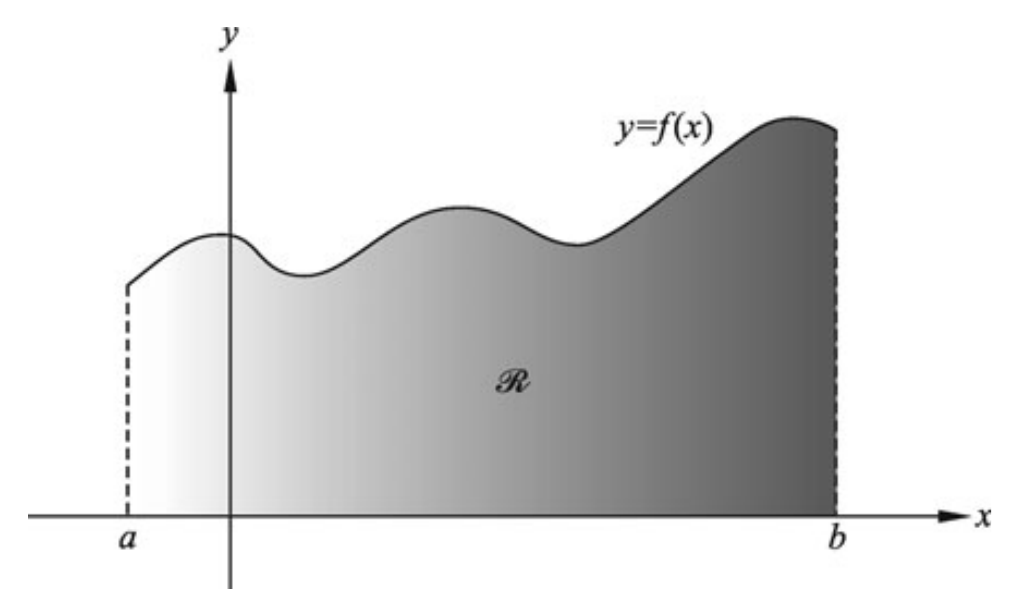
\includegraphics[height=3cm,keepaspectratio=true]{./calculo/fig3001.png}
 % fig3001.png: 0x0 pixel, 300dpi, 0.00x0.00 cm, bb=
 \caption{Región de revolución}
 \label{fig:3001}
\end{figure}




\begin{problema}
 Grafique la superficie de revoluci\'on generada por la regi\'on acotada por la recta $y=x$ y la parábola $y=x^{2}.$
\end{problema}



\begin{observacion}
 A partir de ahora, usaremos el sistema algebráico de computo \texttt{SageMath,} para visualizar las gráficas. 
\end{observacion}



[fragile]{C\'odigo para graficar en 2D}
\begin{verbatim}
x = var("x")
line = x
parabola = x^2
graf = plot(line, (-0.5,1.5))
graf = graf+plot(parabola, (-0.5,1.5))
graf.show()
\end{verbatim}



\begin{figure}
 \centering
 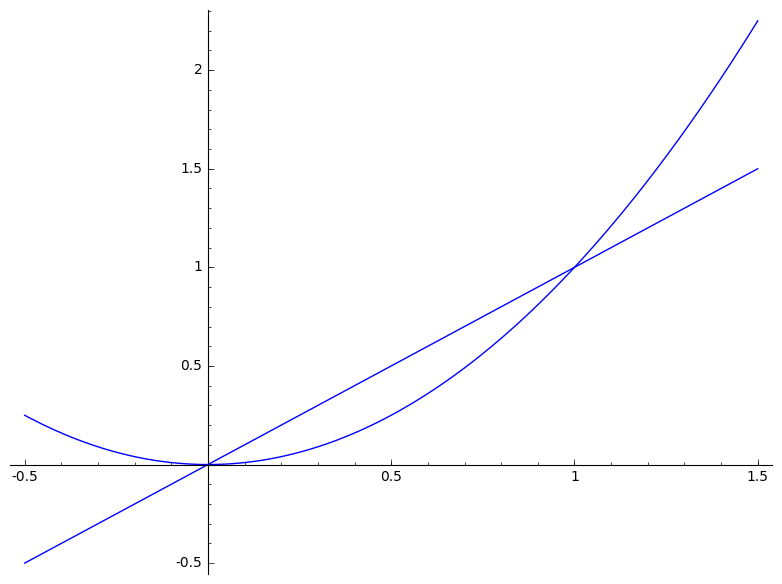
\includegraphics[height=5cm,keepaspectratio=true]{./calculo/sage0501.png}
 % sage0501.png: 0x0 pixel, 300dpi, 0.00x0.00 cm, bb=
 \caption{Regi\'on $\reg$ acotada por $y=x$ y $y=x^{2}$}
 \label{fig:sage:0501}
\end{figure}



[fragile]{C\'odigo para generar un s\'olido de revoluci\'on}
\begin{verbatim}
x = var("x")
line = x
parabola = x^2
P = axes(1, color="black")
sur1=revolution_plot3d(line,(x,0,1),
    opacity=0.5,rgbcolor=(1,0.5,0),
    show_curve=True,parallel_axis='x')
sur2=revolution_plot3d(parabola,(x,0,1),
    opacity=0.5,rgbcolor=(0,1,0),
    show_curve=True,parallel_axis='x')
(sur1+sur2+P).show()
\end{verbatim}




\begin{figure}
 \centering
 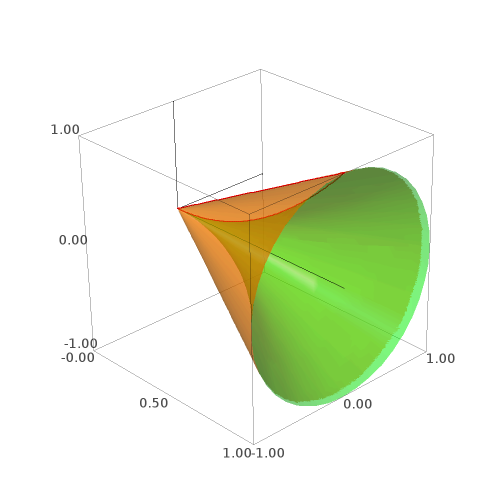
\includegraphics[height=5cm]{./calculo/sage0502.png}
 % sage0502.png: 0x0 pixel, 300dpi, 0.00x0.00 cm, bb=
 \caption{S\'olido generado por $\reg$}
 \label{fig:sage:0502}
\end{figure}



\subsection{F\'ormula del Disco}

El volumen $V$ de un s\'olido de revoluci\'on obtenido al rotar una regi\'on $\reg$ alrededor del eje $x$ está dado por
\[
 \label{disk:formula}
 \tag{F\'ormula del Disco}
 V= \pi \int_{a}^{b}\left( f(x) \right)^{2}dx
\]



\begin{wrapfigure}{l}{2in}
%%%%%%%%%%%%%%%%%%%%%%%%%%%%%%%%%%%%%%%%%%%%%%%%%%%%%%%%%%%%%%%%%%%%%%%%%%%%%%%%%%%%%%%
%%% You will need to add \usepackage{wrapfig} to your preamble to use textwrapping %%%
%%%%%%%%%%%%%%%%%%%%%%%%%%%%%%%%%%%%%%%%%%%%%%%%%%%%%%%%%%%%%%%%%%%%%%%%%%%%%%%%%%%%%%%
 \centering
 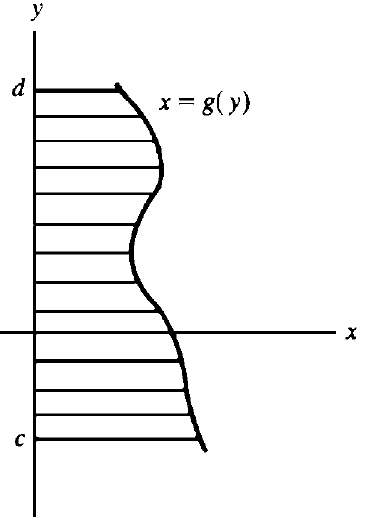
\includegraphics[height=5cm,keepaspectratio=true]{./calculo/fig3003.png}
 % fig3003.png: 0x0 pixel, 300dpi, 0.00x0.00 cm, bb=
 \caption{Regi\'on acotada por $x=g(y)$}
 \label{fig:3003}
\end{wrapfigure} 

De manera similar, la f\'ormula para una regi\'on como acotada por la gráfica $x=g(y)$ está dada por 
\[
 \label{disk:formula:2}
 \tag{F\'ormula del Disco (II)}
 V= \pi \int_{c}^{d}\left( g(y) \right)^{2}dy
\]




\begin{problema}
\begin{wrapfigure}{l}{2.5in}
 \centering
 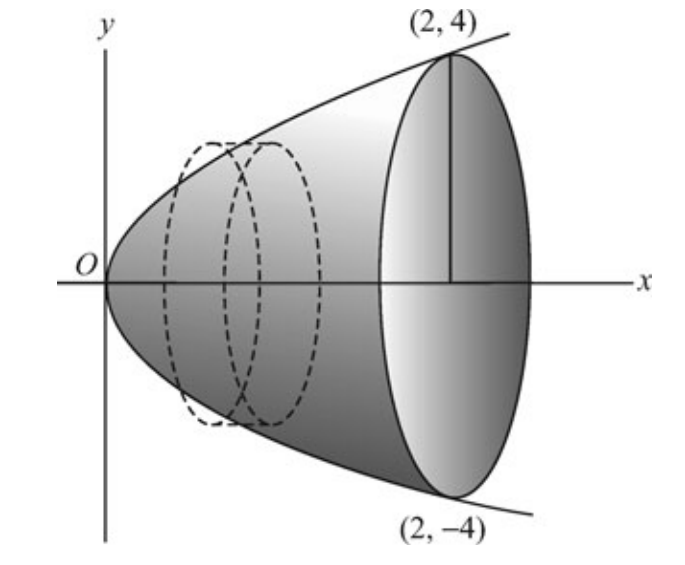
\includegraphics[height=5cm,keepaspectratio=true]{./calculo/fig3004.png}
 % fig3004.png: 0x0 pixel, 300dpi, 0.00x0.00 cm, bb=
 \label{fig:3004}
\end{wrapfigure}

 Considere el s\'olido de revoluci\'on obtenido al girar alrededor del eje $x$ la regi\'on en el primer cuadránte acotada por la parábola  $y^{2}=8x$ y la l\'inea $x=2.$ Encuentre su volumen. 
\end{problema}




\begin{problema}
\begin{wrapfigure}{l}{2.5in}
 \centering
 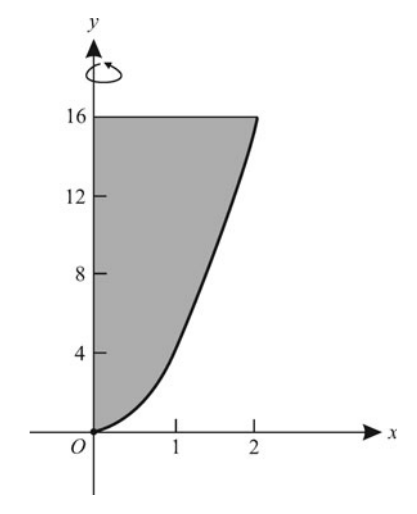
\includegraphics[height=5cm,keepaspectratio=true]{./calculo/fig3005.png}
 % fig3005.png: 0x0 pixel, 300dpi, 0.00x0.00 cm, bb=
 \label{fig:3005}
\end{wrapfigure}

  Considere el s\'olido de revoluci\'on obtenido al girar alrededor del eje $y$ la regi\'on en el primer cuadránte acotada por la parábola  $y=4x^2$ y la l\'inea $y=16.$ Encuentre su volumen. 
\end{problema}



\subsection{M\'etodo de Washer}


\begin{wrapfigure}{l}{2in}
 \centering
 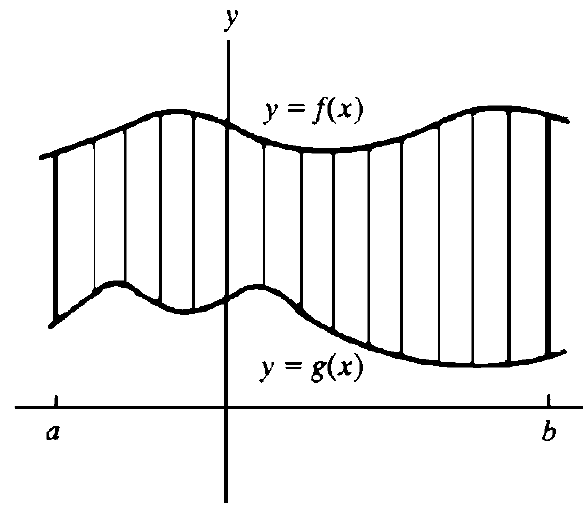
\includegraphics[height=4cm]{./calculo/fig3006.png}
 % fig3006.png: 0x0 pixel, 300dpi, 0.00x0.00 cm, bb=
 \label{fig:3006}
\end{wrapfigure}

Supongamos que $0\leq g(x) \leq f(x)$ para $a\leq x \leq b.$ Consideremos la regi\'on acotada por $x=a,$ $x=b,$ y las curvas $y=g(x)$ y $y=f(x).$ 

Entonces el volumen $V$ del s\'olido de revoluci\'on generado por esta regi\'on rotando alrededor del eje $x$ está dado por 
\[
 \label{washer}
 \tag{Washer}
 V=\pi\int_{a}^{b}\left( (f(x))^{2}-(g(x))^{2} \right)dx
\]




Una f\'ormula similar
\[
 \label{washer:2}
 \tag{Washer (II)}
 V=\pi\int_{c}^{d}\left( (f(y))^{2}-(g(y))^{2} \right)dy
\]
se satisface cuando la regi\'on esta acotada por las curvas $x=f(y),$ $x=g(y)$ y las rectas $y=c,\; y=d,$ siempre y cuando $0\leq g(y) \leq f(y)$ para $c\leq y \leq d$ y se rota tal regi\'on alrededor del eje $y.$



\begin{problema}
 \label{exmp:30.3}
 Considere el s\'olido de revoluci\'on obtenido al girar  alrededor del eje $x$ la regi\'on acotada por las curvas $$y=4x^{2}, \; x=0, \;y=16.$$ 

Encuentre el volumen por \eqref{washer}.
\end{problema}




\begin{figure}
 \centering
 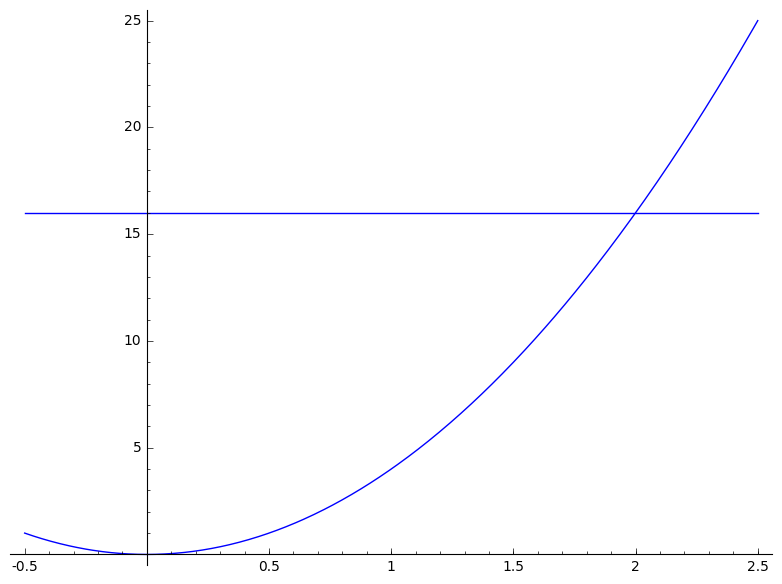
\includegraphics[height=5cm]{./calculo/sage0503.png}
 % sage0503.png: 0x0 pixel, 300dpi, 0.00x0.00 cm, bb=
 \caption{Regi\'on $\reg$ acotada por $y=4x^{2}, \; x=0, \;y=16.$}
 \label{fig:sage:0503}
\end{figure}




\begin{figure}
 \centering
 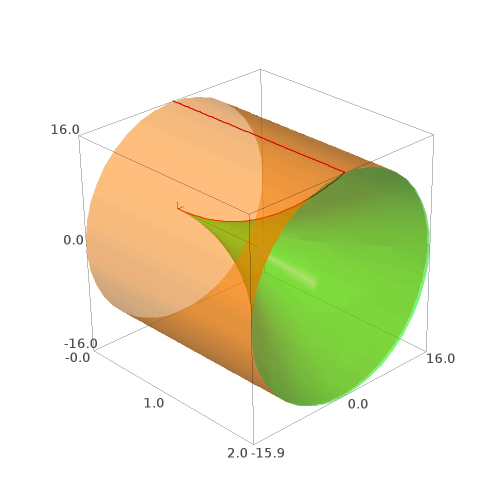
\includegraphics[height=7cm]{./calculo/sage0504.png}
 % sage0503.png: 0x0 pixel, 300dpi, 0.00x0.00 cm, bb=
 \caption{S\'olido generado por regi\'on $\reg.$}
 \label{fig:sage:0504}
\end{figure}



\subsection{M\'etodo de las capas cil\'indricas}


\begin{wrapfigure}{l}{2in}
 \centering
 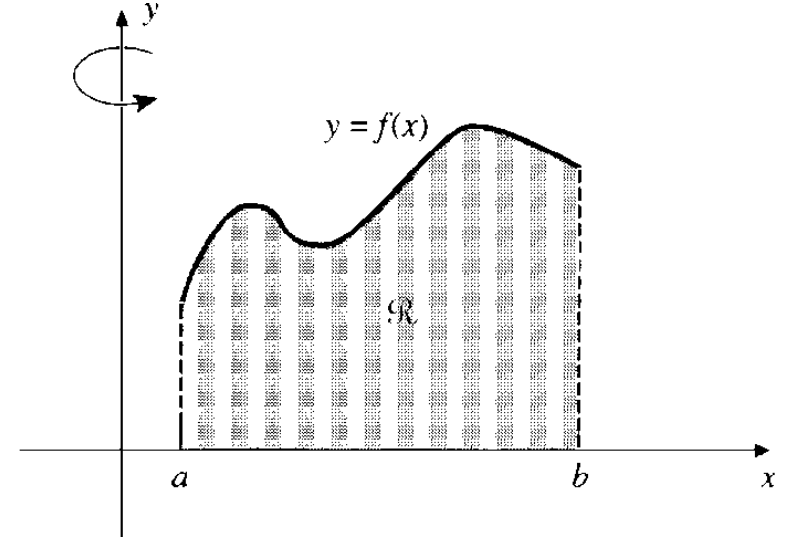
\includegraphics[height=3cm,keepaspectratio=true]{./calculo/fig3007.png}
 % fig3007.png: 0x0 pixel, 300dpi, 0.00x0.00 cm, bb=
 \label{fig:3007}
\end{wrapfigure}

Consideremos el s\'olido de revoluci\'on obtenido al rotar alrededor del eje $y$ la regi\'on $\reg$ en el primer cuadrante entre el eje $x$ y la curva $y=f(x),$ entre $x=a$ y $x=b.$ 

Entonces el volumen del s\'olido está dado por la f\'ormual de capas cil\'indricas
\[
 \label{FCC}
 \tag{FCC}
 V=2\pi \int_{a}^{b}xf(x)dx
\]




Una f\'ormula similar se satisface cuando se intercambian $x$ y $y,$ es decir, la regi\'on $\reg$ en el primer cuadránte entre el eje $y$ y la curva $x=f(y),$ entre $y=c$ y $y=d,$ se gira alrededor del eje $x$
\[
 \label{FCC:2}
 \tag{FCC(II)}
 V=2\pi \int_{c}^{d}yf(y)dy
\]



\begin{problema}
\begin{wrapfigure}{l}{3in}
 \centering
 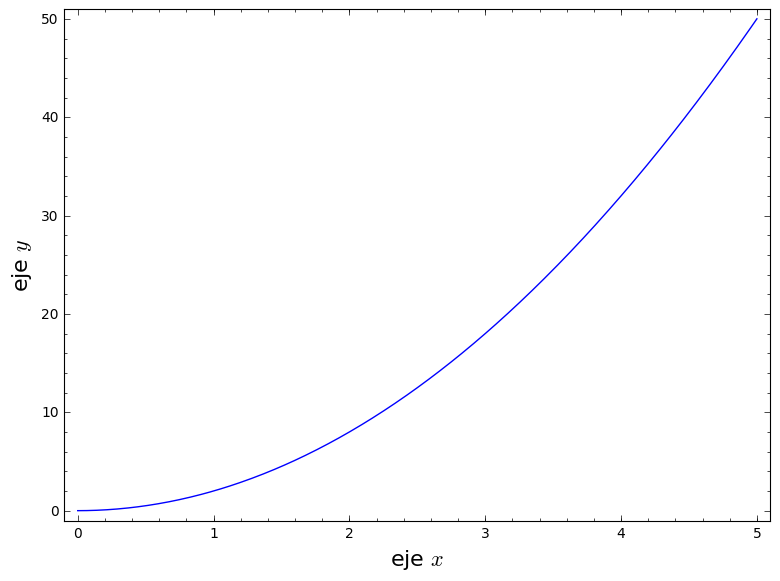
\includegraphics[height=5cm,keepaspectratio=true]{./calculo/sage0505.png}
 % sage0505.png: 0x0 pixel, 300dpi, 0.00x0.00 cm, bb=
 \label{fig:sage:0505}
\end{wrapfigure}

Rote alrededor del eje $y$ la regi\'on sobre el eje $x$ y debajo de $y=2x^{2},$ entre $x=0$ y $x=5.$ Por medio de \eqref{FCC}. Encuentre el volumen.
\end{problema}



\begin{figure}
 \centering
 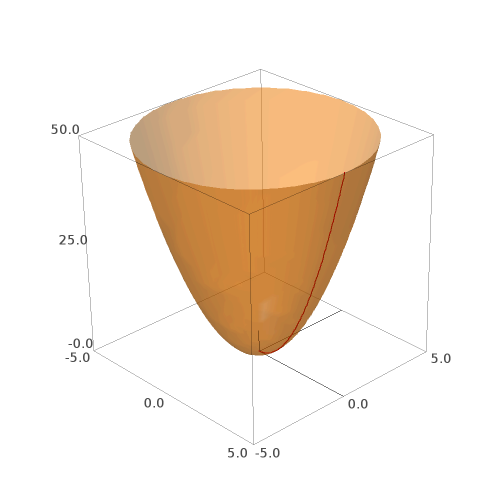
\includegraphics[height=7cm,keepaspectratio=true]{./calculo/sage0506.png}
 % sage0506.png: 0x0 pixel, 300dpi, 0.00x0.00 cm, bb=
 \label{fig:sage:0506}
\end{figure}



\subsection{Diferencia de Capas}


Supongamos que $0\leq g(x) \leq f(x)$ en el intervalo $[a,b], \; a \geq 0.$ Sea $\reg$ la regi\'on en el primer cuadránte entre $$y=f(x), \; y=g(x), \; x=a, \; x=b.$$ 

Entonces el volumen del s\'olido de revoluci\'on obtenido al rotar $\reg$ alrededor del eje $y$ está dado por
\[
 \label{FDC}
 \tag{FDC}
 V=2\pi\int_{a}^{b}x\left( f(x)-g(x) \right)dx
\]




\begin{problema}
\begin{wrapfigure}{l}{2.5in}
 \centering
 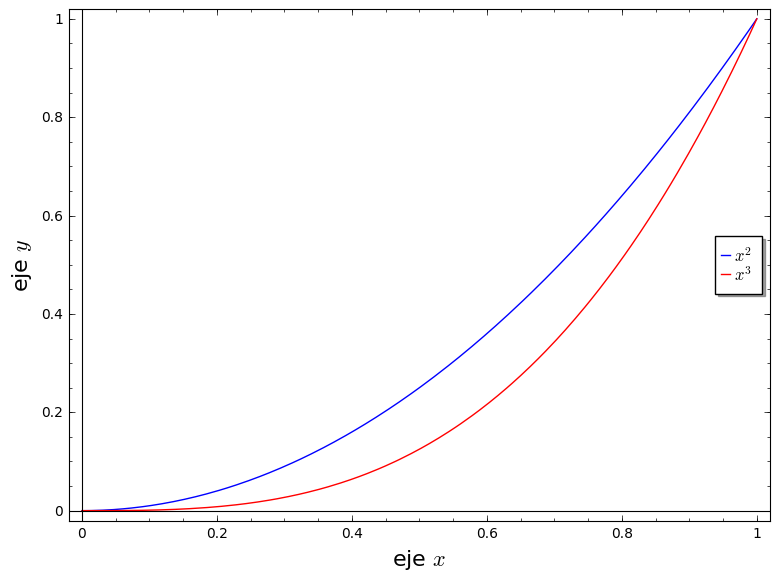
\includegraphics[height=5cm,keepaspectratio=true]{./calculo/sage0507.png}
 % sage0507.png: 0x0 pixel, 300dpi, 0.00x0.00 cm, bb=
 \label{fig:sage:0507}
\end{wrapfigure}


 Consideremos la regi\'on en el primer cuadrante acotado arriba por $y=x^{2}$ y debajo por $y=x^{3}.$

Encuentre el volumen del s\'olidos generado al rotar $\reg$ alrededor del eje $y.$
\end{problema}




\begin{figure}
 \centering
 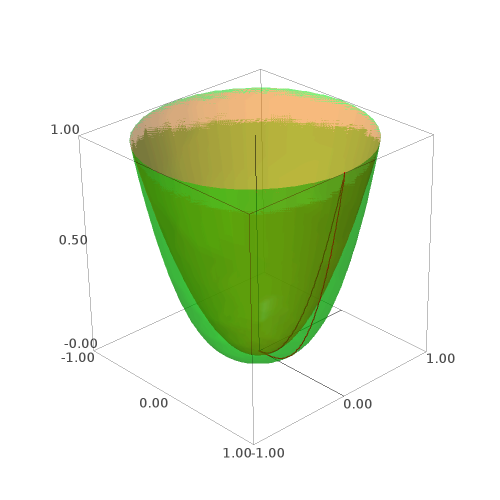
\includegraphics[height=7cm,keepaspectratio=true]{./calculo/sage0508.png}
 % sage0508.png: 0x0 pixel, 300dpi, 0.00x0.00 cm, bb=
 \label{fig:sage:0508}
\end{figure}



\subsection{Secciones trasnversales (rebanadas)}


\begin{wrapfigure}{l}{3.5in}
 \centering
 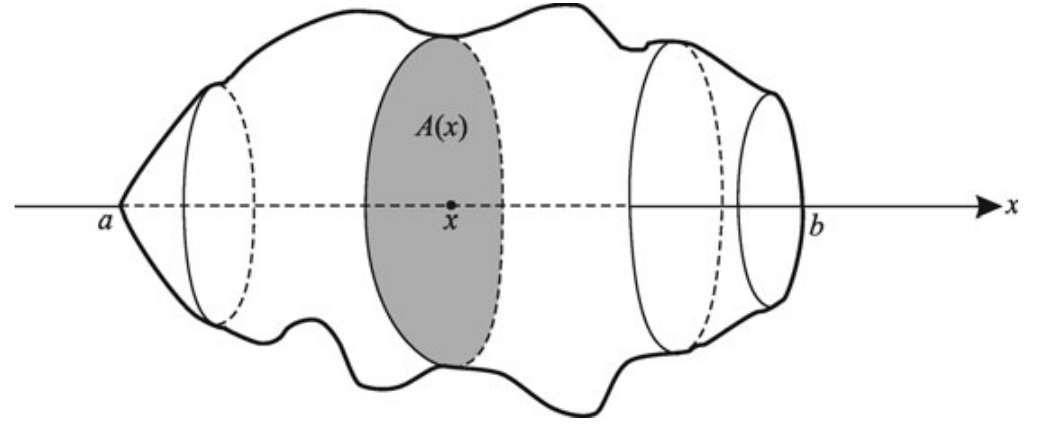
\includegraphics[height=3cm,keepaspectratio=true]{./calculo/fig3008.png}
 % fig3008.png: 0x0 pixel, 300dpi, 0.00x0.00 cm, bb=
 \label{fig:3008}
\end{wrapfigure}


Supongamos que un s\'olido vive enteramente entre el plano perpendicular al eje $x$ en $x=a$ y el plano perpendicular al  $x$ en $x=b.$ 

Para cada $x\in [a,b],$ supongamos que el plano perpendicular al eje $x$ en el punto $x$ intersecta al s\'olido en una regi\'on de área $A(x).$



Entonces, el volumen $V$ del s\'olido está dado por 
\[
 \label{fst}
 \tag{FST}
 V=\int_{a}^{b}A(x)dx.
\]


\begin{problema}
\begin{wrapfigure}{l}{6cm}
 \centering
 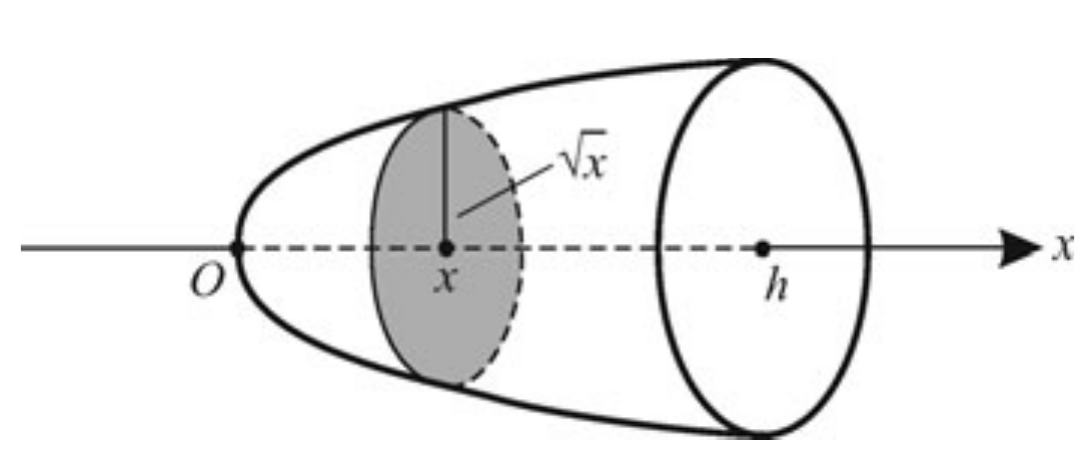
\includegraphics[width=5cm,keepaspectratio=true]{./calculo/fig3009.png}
 % fig3009.png: 0x0 pixel, 300dpi, 0.00x0.00 cm, bb=
 \label{fig:3009}
\end{wrapfigure}

 Supongamos que un segmento de un misil de longitud $h$ es tal que la secci\'on transversal perpendicular al eje de simetr\'ia del misil a una distancia $x$ de la punta  es un c\'irculo de radio $\sqrt{x}.$ Encuentre el volumen del misil.
\end{problema}



\section{Integrales impropias}

\subsection{L\'imites al infinito}


Para que $$\displaystyle\int_{a}^{b}f(x)dx$$ est\'e bien definida, basta que $f$ sea una funci\'on continua y $a,b$ sean número reales. Ahora veremos que sucede cuando
\begin{enumerate}
 \item  $a$ o $b$ tienden a $\pm \infty;$
 \item $f$ es discontinuo.
\end{enumerate}

Tales integrales se conocen como \emph{impropias.}
 

{L\'imites infinitos de integraci\'on}
\begin{align}
\label{35.a}
 \displaystyle\int_{a}^{+\infty}f(x)dx &= \lim_{c\to +\infty} \int_{a}^{c}f(x)dx \\
\label{35.b}
 \displaystyle\int_{-\infty}^{b}f(x)dx &= \lim_{c\to -\infty} \int_{c}^{b}f(x)dx \\
 \label{35.c}
 \int_{-\infty}^{+\infty}f(x)dx &= \int_{c}^{+\infty}f(x)dx+\int_{-\infty}^{c}f(x)dx
\end{align}
La última integral es válida siempre y cuando los dos l\'imites del lado derecho existan.



\begin{problema}
\label{solved:35.6}
 Encuentre la intergral 
 $$\displaystyle \int_{0}^{\infty}e^{-x}\sin(x) dx$$
\end{problema}




\begin{problema}
 \label{solved:35.4}
Encuentre la integral
$$\displaystyle \int_{-\infty}^{0} e^{rx}dx$$ para $r>0.$
\end{problema}




\begin{problema}
 \label{solved:35.7}
Evalue 
$$
\displaystyle \int_{-\infty}^{\infty}
\dfrac{dx}{e^{x}+e^{-x}}
$$
\end{problema}


\subsection{Discontinuidades del integrando}

{Caso I}
Si $f$ es continuo en $(a,b],$ discontinuo en $x=a,$ podemos definir
$$
\displaystyle \int_{a}^{b}f(x)dx=\lim_{u\to a^{+}} \int_{u}^{b}f(x)dx,
$$ siempre y cuando el l\'imite exista.


\begin{problema}
 Evalue
 $$\displaystyle \int_{0}^{1}\dfrac{dx}{x^{2}} dx$$
\end{problema}



{Caso II}
Si $f$ es continuo en $[a,b),$ discontinuo en $x=b,$ podemos definir
$$
\displaystyle \int_{a}^{b}f(x)dx=\lim_{u\to b^{-}} \int_{a}^{u}f(x)dx,
$$ siempre y cuando el l\'imite exista.


\begin{problema}
 Evalue
 $$\displaystyle \int_{0}^{\pi/2}\dfrac{\cos(x)}{\sqrt{1-\sin(x)}} dx$$
\end{problema}



{Caso III}
Si $f$ es continuo en $[a,b]$ excepto en un punto $c\in(a,b),$ entonces
$$
\int_{a}^{b}f(x)dx = 
\lim_{u \to c^{-}} \int_{a}^{u}f(x)dx+
\lim_{u \to c^{+}} \int_{u}^{b}f(x)dx
$$
siempre y cuando ambos l\'imites del lado derecho existan.


\begin{problema}
 Evalue 
$$\displaystyle \int_{0}^{4}\dfrac{dx}{\sqrt[3]{x-1}} dx$$
\end{problema}


\section{Área de Superficies de Revoluci\'on}


Si un arco de una curva se gira alrededor de una l\'inea que no se intersecta con el arco, entonces la superficie resultante is llamada \emph{superficie de revoluci\'on.} 

Por \emph{área de superficie,} nos referiremos al área de la superficie exterior.




Sea $f$ una funci\'on continua y $f(x)\geq 0$  en $[a,b]$ que es diferenciable en $(a,b).$  Entonces el área de superficie $S$ de la superficie de revoluci\'on  generado al girar la gráfica de $f$ en $[a,b]$ alrededor del eje $x$ esta dado por la f\'ormula
\[
 \label{36.1}
 S=2\pi \int_{a}^{b}f(x)\sqrt{1+(f'(x))^{2}}dx.
\]





De manera similar, sea $g$ una funci\'on continua y $g(y) \geq 0$  en $[c,d]$ que es diferenciable en $(c,d).$  Entonces el área de superficie $S$ de la superficie de revoluci\'on  generado al girar la gráfica de $g$ en $[c,d]$ alrededor del eje $y$ esta dado por la f\'ormula
\[
 \label{36.2}
 S=2\pi \int_{c}^{d}g(y))\sqrt{1+(g'(y))^{2}}dy.
\]




De manera más general, si una curva esta dada por las ecuaciones param\'etricas
$$
x=f(u), \; y=g(u)
$$ y el arco va de $u=u_{1}$ a $u=u_{2}$ se rota alrededor del eje $x,$ entonces el área de superficie de la superficie de revoluci\'on resultante está dada por la f\'ormula
\[
 \label{36.3}
 S=2\pi\int_{u_{1}}^{u_{2}}y\sqrt{\left( \dfrac{dx}{du} \right)^{2}+\left( \dfrac{dy}{du} \right)^{2}}du
\]
 

En la f\'ormula anterior, hemos supuesto que $f,g$ son continuas en $[u_{1},u_{2}],$ diferenciable en $\left( u_{1},u_{2} \right)$ y que $y=g(u)\geq 0$ en $[u_{1},u_{2}].$
